\documentclass[10pt,a4paper]{article}
\usepackage[margin=13mm,top=12mm,bottom=14mm]{geometry}
\usepackage{graphicx,xcolor,tabularx,booktabs,array,enumitem,microtype,lmodern,fancyhdr,tikz}
\usepackage[T1]{fontenc}
\usetikzlibrary{arrows.meta,positioning,shapes.geometric}
\setlength{\parindent}{0pt}\setlength{\parskip}{3pt}
\sloppy
\setlist{leftmargin=5mm,itemsep=1pt,topsep=2pt}
\definecolor{navy}{HTML}{17365D}\definecolor{blue}{HTML}{2F75B5}
\definecolor{green}{HTML}{548235}\definecolor{amber}{HTML}{BF8F00}
\definecolor{red}{HTML}{C00000}\definecolor{gray}{HTML}{666666}
\definecolor{pb}{HTML}{E7F0F8}\definecolor{pg}{HTML}{EAF2E3}
\definecolor{pa}{HTML}{FFF3D6}\definecolor{pr}{HTML}{FBE5E5}\definecolor{px}{HTML}{EEEEEE}
\newcommand{\boxx}[2]{\colorbox{#1}{\parbox{\dimexpr\linewidth-2\fboxsep}{#2}}}
\newcommand{\headx}[1]{{\color{navy}\LARGE\bfseries #1}\par\vspace{1mm}{\color{blue}\rule{\linewidth}{1.1pt}}\vspace{2mm}}
\newcommand{\status}[2]{\colorbox{#1}{\textcolor{white}{\bfseries\scriptsize #2}}}
\newcommand{\pass}{\status{green}{PASS}}\newcommand{\supported}{\status{green}{SUPPORTED}}
\newcommand{\hold}{\status{amber}{HOLD}}\newcommand{\fail}{\status{red}{FAIL}}
\newcommand{\unresolved}{\status{gray}{UNRESOLVED}}\newcommand{\notclaimed}{\status{gray}{NOT YET CLAIMED}}
\pagestyle{fancy}\fancyhf{}\lhead{\footnotesize Detailed supervisor progress report}
\rhead{\footnotesize 11 August 2026}\cfoot{\footnotesize\thepage\ / 13}\renewcommand{\headrulewidth}{.3pt}
\begin{document}

\headx{Technical Progress Report}
{\Large\bfseries Mode-II Reference Verification, Adaptive Remeshing,\par State Transfer, and Parallelization Assessment\par for Phase-Field Fracture in Abaqus\par}
\begin{tabularx}{\linewidth}{@{}lX@{}}
\textbf{Author} & Pruthviraja Reddy Vandavagali\\
\textbf{Programme} & Master Thesis, TU Bergakademie Freiberg\\
\textbf{Date} & 11 August 2026\\
\textbf{Objective} & Accurate phase-field fracture with locally refined meshes, controlled state transfer, and a defensible computational-cost reduction.\\
\end{tabularx}
\boxx{pb}{\textbf{Progress since the 24 July report.} The earlier Mode-I development story remains valid in its stated scope. Since then, the work has moved to a Mode-II verification/production branch: a corrected H0/H1/H2 study, two endpoint-complete adaptive MM/PK5 runs, and a state-transfer restart investigation. A later executable-path audit overturned the initial restart interpretation: the transfer artifact existed, but the running UEL did not consume it.}
\boxx{pg}{\textbf{Major supported result.} A scientifically identical H2 rerun removed the PBS-walltime ambiguity: it reproduced the historical trajectory exactly to $u_1=0.009250$ mm, developed an interior peak, and then stopped by genuine nonlinear divergence. H1/H2 remain closely aligned over their enlarged common domain.}
\boxx{pr}{\textbf{Current evidence boundary.} Crack-path convergence fails its frozen matched-state gate. Runtime state ingestion fails. A second evolving remesh, general thread safety, MPI/hybrid safety, and an online adaptive-remesh loop are not established.}
\small
\begin{tabularx}{\linewidth}{@{}XrXr@{}}\toprule
Pre-peak uniform verification&\pass&Adaptive MM/PK5 production&\pass\\
Adaptive global response&\supported&Matched-state crack path&\fail\\
Nonmatching transfer artifact&\supported&Mechanical re-equilibration claim&\fail\\
Runtime state ingestion&\fail&Second evolving remesh&\hold\\
Parallel thread safety&\unresolved&MPI / hybrid safety&\unresolved\\
Online adaptive remeshing&\notclaimed&Thesis integration&\supported\\\bottomrule
\end{tabularx}
\boxx{pb}{\textbf{H2 endpoint-resolution result.} The 24-hour-envelope run reached $u_1=0.0097625$ mm in 15,990 s walltime, then terminated because the solution was judged unlikely to converge and the fixed increment was too large. Scheduler limitation is no longer the reason H2 is incomplete. Global H0/H1/H2 peak convergence nevertheless remains unresolved because H1 is terminally incomplete.}
\vfill\footnotesize Report evidence revisions: endpoint closeout \texttt{0b36c8ed}; final report revision recorded in repository history.

\clearpage\headx{1. From Mode I development to Mode II verification}
The 24 July report documented the Mode-I development benchmark, layered UEL/UMAT/UEXTERNALDB architecture, MISESERI-guided offline refinement, bounded transfer, fixed-active-set failure, and offline KKT correction. None of that evidence is invalidated. The present Mode-II branch is a later, more demanding verification and adaptive-production benchmark that retains the same methodology: one physical mesh reconstructed as coincident phase, mechanics, and visualization layers; deterministic packages; and claim-by-claim validation.

The Mode-II specimen uses split notch faces and horizontal shear loading. The qualified FRACFIX formulation uses $l_0=0.015$ mm, $G_c=0.0027$ kN/mm, $E=210$ kN/mm$^2$, $\nu=0.3$, unit thickness, and residual stiffness $k=10^{-7}$. Four-node and three-node elements are supported in three coincident logical layers. U1 is the quadrilateral phase-field UEL, U2 the quadrilateral displacement UEL, U3 the triangular phase-field UEL, and U4 the triangular displacement UEL. Separate passive CPE4/CPE3 facsimile elements form the output layer.

The current producer contract is: SDV14 carries the phase used by the mechanical U2/U4 layer; SDV15 is the current solved phase from U1/U3; and SDV16 is history $H$ from the mechanical/history path. SDV14 and SDV15 may differ during staggered execution.

\begin{center}
\resizebox{.90\linewidth}{!}{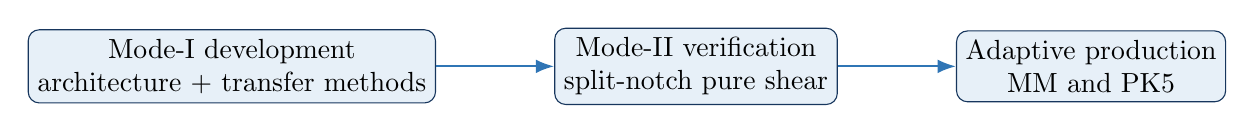
\begin{tikzpicture}[node distance=15mm,box/.style={draw=navy,rounded corners,fill=pb,minimum width=34mm,minimum height=9mm,align=center},arr/.style={-{Latex},thick,blue}]
\node[box] (m1) {Mode-I development\\architecture + transfer methods};
\node[box,right=of m1] (m2) {Mode-II verification\\split-notch pure shear};
\node[box,right=of m2] (m3) {Adaptive production\\MM and PK5};
\draw[arr] (m1)--(m2);\draw[arr](m2)--(m3);
\end{tikzpicture}}
\\[-1mm]\footnotesize Method continuity $\rightarrow$ verified Mode-II branch $\rightarrow$ adaptive production.
\end{center}
\boxx{pa}{\textbf{Reason for the transition.} Mode II supplies the current common reference/adaptive comparison problem and exercises mixed-mode-sensitive localization. It is not a replacement for the Mode-I development evidence; it is the next verification and production branch.}

\clearpage\headx{2. Uniform H0/H1/H2 reference verification}
\small
\begin{tabularx}{\linewidth}{@{}lrrrr@{}}\toprule
Metric&H0&H1&H2&Interpretation\\\midrule
Physical elements&3,930&12,064&33,852&$h/l_0=2.0,1.0,0.5$\\
Valid $u_1$ maximum (mm)&0.010000&0.0096325&0.0097625&H1/H2 common: 0--0.0096325\\
$K_0$ (kN/mm)&46.1396&45.9035&45.8741&H2--H1: $-0.064\%$\\
$u_1(d\geq0.5)$ (mm)&0.008250&0.007750&0.007750&H1/H2 parity\\
H2 vs H1 $L_2$ / work area&--&--&0.536\% / 0.287\%&new common domain\\
Matched RF / $d_{\max}$ difference&--&--&$-1.445\%$ / $+0.001948$&at $u_{\max}^{\rm common}$\\
CPU / wall (s)&2000/2004&5434/5453&15949/15990&measured serial cost\\
Termination&endpoint&divergence&divergence&H1/H2 incomplete\\\bottomrule
\end{tabularx}
\normalsize
Because the original H2 stopped at its four-hour PBS limit, it was repeated without changing its input bytes, UEL, mesh, increments, or parameters, but with a 24-hour scheduler envelope. Job 1388330 reproduced the old RF--U and $d_{\max}$ histories exactly through $u_1=0.009250$ mm (RF $L_2$, work, maximum RF difference, and matched $d_{\max}$ difference all zero). It continued for only 1,489 additional wall seconds, developed an interior peak $RF_1=0.358134$ kN at $u_1=0.009500$ mm, and terminated at $u_1=0.0097625$ mm after Step 2 increment 1906 because the nonlinear solution was judged unlikely to converge and the fixed increment was too large. PBS walltime is therefore excluded as the H2 stopping mechanism.

The enlarged H1/H2 common domain ends at $u_1=0.0096325$ mm. Over it, normalized RF $L_2=0.536\%$, absolute work difference $=0.287\%$, matched RF difference $=-1.445\%$, and matched $d_{\max}$ difference $=+0.001948$. Origin-OLS stiffness differs by only $-0.064\%$. Both reach $d_{\max}\geq0.5$ at 0.00775 mm, whereas $d_{\max}\geq0.9$ occurs at 0.00850 mm for H1 and 0.00800 mm for H2. Thus the pre-peak/near-peak global force response is highly consistent, while later localization timing is more mesh-sensitive.

At matched $u_1=0.009250$ mm the H1/H2 crack sets ($d\geq0.5$) have Hausdorff distance 0.005443 mm, above the frozen 0.003750 mm gate. Thus:
No H2 detailed field frame exists exactly at the new common endpoint; the nearest later H2 frame is approximately 0.0097500 mm and lies outside the H1 domain. No new-endpoint Hausdorff value is therefore claimed. Direct validated phase-field fracture-energy history is unavailable; ALLSE or ALLWK$-$ALLSE is not substituted, and energy convergence remains unresolved.
\begin{center}\begin{tabular}{ll}
pre-peak mesh-refinement consistency & \pass\\damage-initiation consistency&\pass\\
H1 minimum pre-peak/global comparator&\supported\\H2 fine spatial diagnostic&\supported\\
matched-state crack-path convergence&\fail\\global peak convergence&\unresolved\\
full post-peak uniform convergence&\unresolved\\complete uniform fracture reference&\textbf{NONE}
\end{tabular}\end{center}

\clearpage\headx{3. Uniform-reference figures and interpretation}
\begin{center}
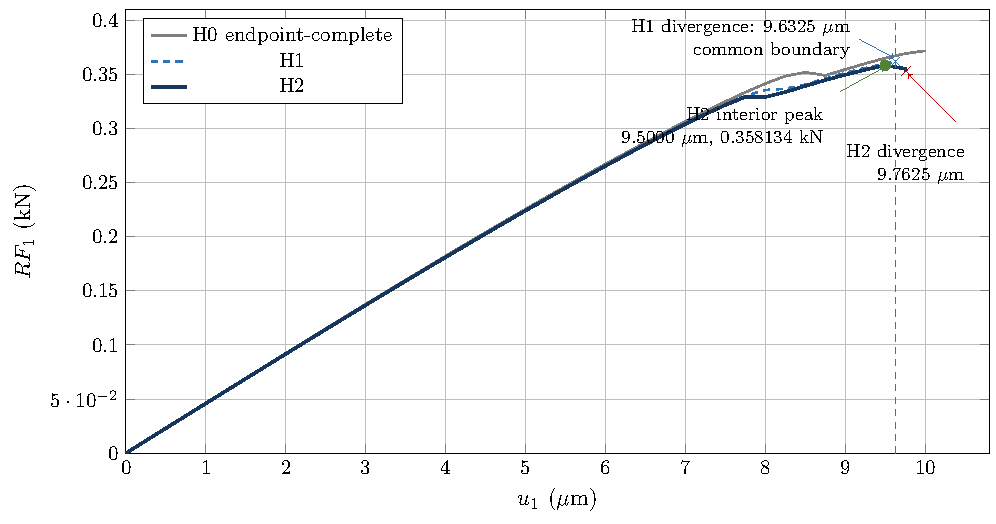
\includegraphics[width=.88\linewidth]{../../results/figures/mode_ii_reference_convergence/mode_ii_h0_h1_h2_rf1_u1_comparison.pdf}\\[-1mm]
\footnotesize\textbf{Figure 1.} RF1--U1 comparison from primary extracted curves. H2 reproduces its historical trajectory exactly to 0.00925 mm, reaches an interior peak at 0.00950 mm, and then diverges numerically at 0.0097625 mm. H1 diverges at 0.0096325 mm; hence global H1/H2 peak convergence remains unresolved.\\[2mm]
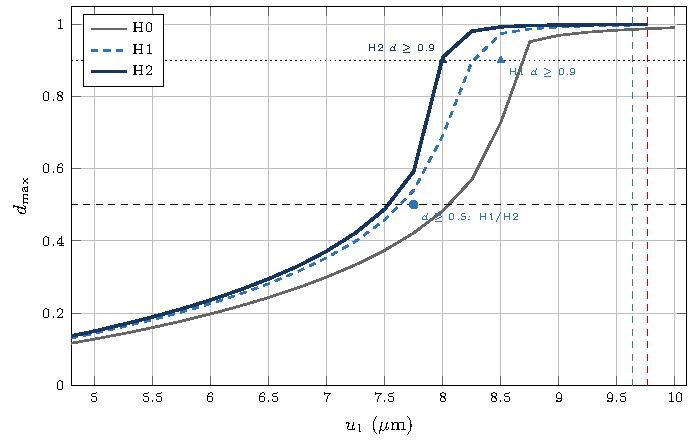
\includegraphics[width=.48\linewidth]{../../results/figures/mode_ii_reference_convergence/mode_ii_h0_h1_h2_damage_evolution_comparison.pdf}\hfill
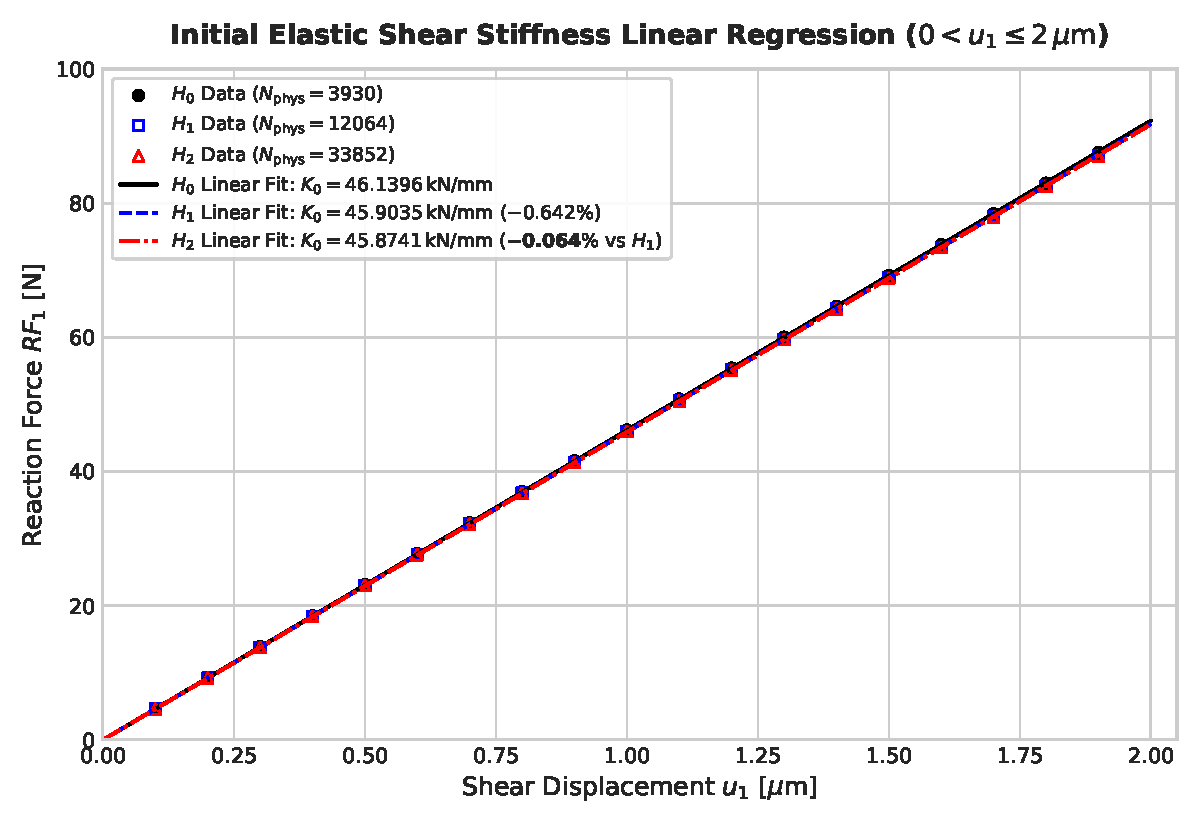
\includegraphics[width=.48\linewidth]{../../results/figures/mode_ii_reference_convergence/mode_ii_h0_h1_h2_initial_stiffness_fit.pdf}\\[-1mm]
\footnotesize\textbf{Figures 2--3.} Extended damage evolution and identical origin-OLS stiffness over $0<u_1\leq0.002$ mm. H1/H2 share $d_{\max}\geq0.5$ initiation at 0.00775 mm; $d_{\max}\geq0.9$ shifts from 0.00850 mm (H1) to 0.00800 mm (H2). $K_0=$46.1396, 45.9035, and 45.8741 kN/mm for H0/H1/H2.
\end{center}
\normalsize H2's global phase range is 0 to 0.999966 with no overshoot. SDV16 has no negative transitions, but eight small SDV15 decreases occur (worst $-3.9768\times10^{-4}$). History monotonicity is supported; strict solved-phase pointwise irreversibility is not established.

\clearpage\headx{4. Adaptive mesh development and production}
MISESERI pre-analysis was used to localize resolution before the fracture solves. MM (MINIMUM\_MAXIMUM sizing) contains 2,206 physical elements and concentrates refinement strongly, with crack-corridor median $h/l_0=0.8170$. PK5 (5\% UNIFORM\_ERROR target) contains 4,894 physical elements and provides denser corridor coverage, median $h/l_0=0.6033$. Both were carried forward because mesh statistics alone could not select a scientific winner.
\small
\begin{tabularx}{\linewidth}{@{}p{18mm}p{14mm}p{19mm}p{26mm}XX@{}}\toprule
Job&Elements&CPU / wall&Peak RAM / VMEM&Solver result&Scope\\\midrule
MM 1386469&2,206&164 / 166 s&4.86 / 7.58 GB&endpoint, 2,500 increments, 0 cutbacks&lower-cost localization\\
PK5 1386470&4,894&366 / 368 s&10.12 / 12.90 GB&endpoint, 2,500 increments, 0 cutbacks&higher corridor resolution\\\bottomrule
\end{tabularx}
\normalsize Both jobs completed at $u_1=0.010000$ mm with exit status 0. The retained comparison reports approximately 0.16\% maximum relative RF difference between MM and PK5. This is strong adaptive-to-adaptive \emph{global-response} agreement; it is not evidence of crack-path convergence. Energy outputs were requested, but no new energy-convergence claim is made here without a completed combined field/energy closeout.
\boxx{pg}{\textbf{Supported result.} Two materially different adaptive meshes completed the full prescribed displacement and produced very close RF--U response.}
\boxx{pa}{\textbf{Boundary.} Spatial fracture agreement and a final adaptive winner remain separate questions.}

\clearpage\headx{5. Accuracy versus measured serial cost}
\begin{center}
\resizebox{.96\linewidth}{!}{%
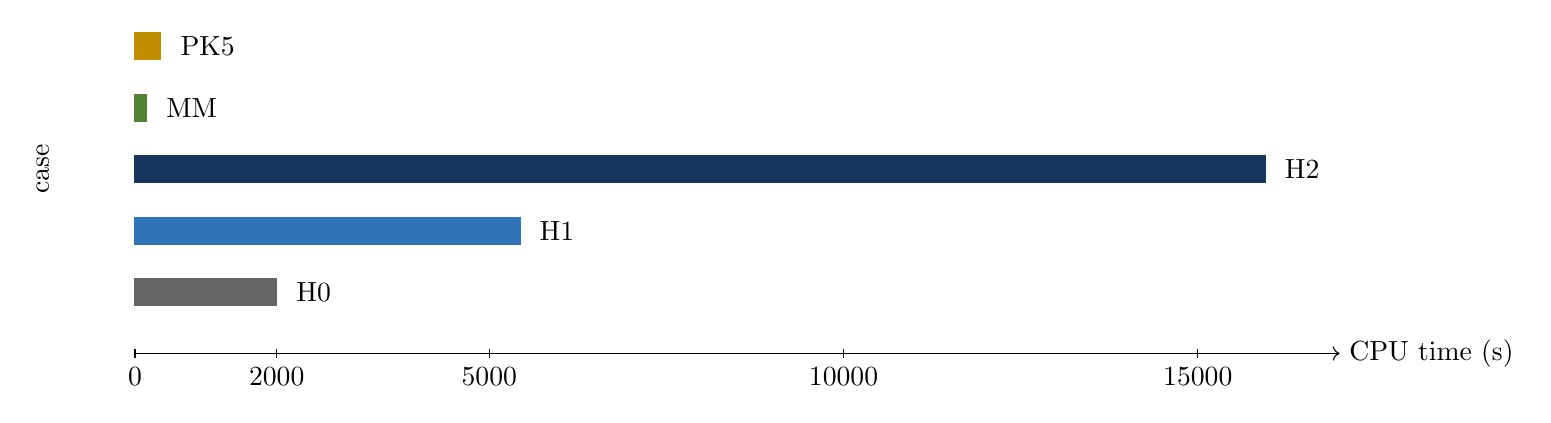
\begin{tikzpicture}[x=0.0009cm,y=.78cm]
\draw[->] (0,0)--(17000,0) node[right]{CPU time (s)};
\foreach \x/\lab in {0/0,2000/2000,5000/5000,10000/10000,15000/15000}{\draw (\x,0.08)--(\x,-0.08) node[below]{\lab};}
\foreach \x/\y/\name/\col in {2000/1/H0/gray,5434/2/H1/blue,15949/3/H2/navy,164/4/MM/green,366/5/PK5/amber}{\draw[fill=\col,draw=\col] (0,\y-.22) rectangle (\x,\y+.22);\node[anchor=west] at (\x+140,\y){\name};}
\node[rotate=90] at (-1300,3){case};
\end{tikzpicture}
}
\end{center}
\footnotesize\raggedright\textbf{Figure 4.} Audited CPU time for H0/H1/H2 and endpoint-complete MM/PK5, all one-CPU Abaqus 2023 executions. Accuracy is not encoded as a censored peak metric; the accompanying table states the valid response evidence. Sources: uniform censoring audit and jobs 1386469--1386470.\par
\small
\begin{tabularx}{\linewidth}{@{}lrrX@{}}\toprule
Case&CPU vs H2&Elements&Scientifically comparable response statement\\\midrule
H0&7.9745$\times$ lower&3,930&coarse baseline; full endpoint\\
H1&2.9343$\times$ lower&12,064&minimum supported pre-peak comparator; incomplete\\
H2&baseline&33,852&fine spatial diagnostic; numerically incomplete\\
MM&97.25$\times$ lower&2,206&endpoint-complete adaptive run\\
PK5&43.58$\times$ lower&4,894&endpoint-complete adaptive run\\\bottomrule
\end{tabularx}
\normalsize The extended H2 consumed 15,949 s CPU and 15,990 s walltime, versus 14,455/14,501 s historically: only 1,494 additional CPU seconds and 1,489 wall seconds (00:24:49) exposed the genuine numerical termination. Ratios to H2 are measured serial CPU-time ratios, not claims of equivalent complete-fracture accuracy; H1/H2 are incomplete uniform diagnostics, whereas MM/PK5 reached the prescribed endpoint.

\clearpage\headx{6. State transfer and the restart claim audit}
\begin{center}
\resizebox{.72\linewidth}{!}{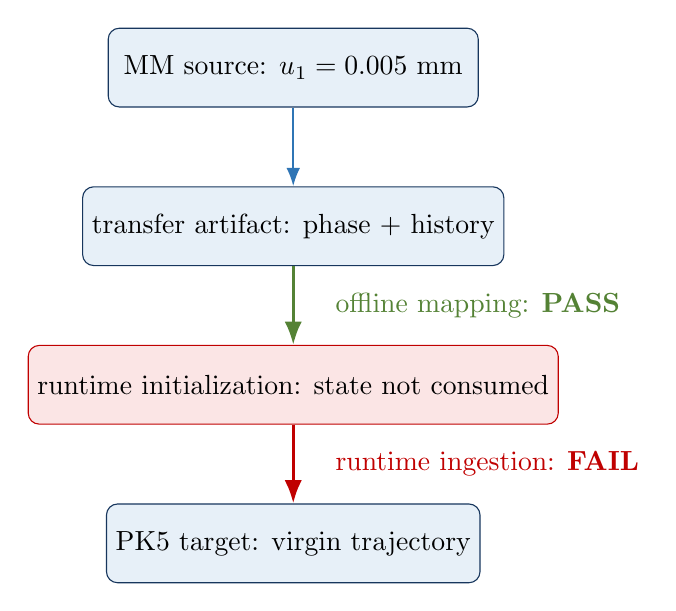
\begin{tikzpicture}[node distance=10mm,box/.style={draw=navy,rounded corners,fill=pb,minimum width=47mm,minimum height=10mm,align=center},bad/.style={draw=red,rounded corners,fill=pr,minimum width=47mm,minimum height=10mm,align=center},arr/.style={-{Latex},thick,blue}]
\node[box](s){MM source: $u_1=0.005$ mm};\node[box,below=of s](a){transfer artifact: phase + history};
\node[bad,below=of a](i){runtime initialization: state not consumed};\node[box,below=of i](t){PK5 target: virgin trajectory};
\draw[arr](s)--(a);\draw[-{Latex},very thick,green](a)--node[right=4mm,text=green]{offline mapping: \textbf{PASS}}(i);\draw[-{Latex},very thick,red](i)--node[right=4mm,text=red]{runtime ingestion: \textbf{FAIL}}(t);
\end{tikzpicture}}
\end{center}
\footnotesize\textbf{Figure 5.} Audited source-to-runtime chain for job 1386471. The artifact exists and offline mapping is traceable, but the executable path does not ingest it. Source: runtime-ingestion audit F43STATE-M2-RUNTIME-INGESTION-AUDIT1.\par
\normalsize
Job 1386471 used MM Step-1 frame 500 ($u_1=0.005000$ mm) as the intended source and a nonmatching PK5 target (4,894 physical; 14,682 layered elements). The artifact contained mapped nodal phase and integration-point history; the offline phase $L_2$ mapping error was 0.048\%, with bounds and coverage checks passing. The target solve then completed to $u_1=0.010000$ mm in 2,100 increments, 4,200 equilibrium iterations, and no cutbacks.

Those facts initially appeared to support a restart. The later audit proved otherwise: \texttt{STATE\_TRANSFER\_ARTIFACT.json} is never read by the solver; the UEL does not read the passed \texttt{SVARS}; mutable \texttt{COMMON/KUSER/USRVAR} starts at zero; and nodal phase also starts at zero. Job 1386471 exactly reproduced the virgin PK5 checkpoint state. Zero RF and ALLSE jumps therefore demonstrate trajectory identity, not successful transferred-state re-equilibration. Observed phase decreases during the nominal re-equilibration (76 locations, maximum 0.1245) further contradict the intended irreversibility claim.
\boxx{pr}{\textbf{Current classification.} Artifact creation and MM-to-artifact trace: SUPPORTED. Artifact-to-running-solver trace: FAIL. Controlled restart and mechanical re-equilibration claims: FAIL. Restart2 checkpoint validity and second evolving-remesh readiness: HOLD.}

\clearpage\headx{7. Parallelization of the ExternalDB / COMMON-block implementation}
\textbf{Supervisor question.} Does using ExternalDB and COMMON blocks still prevent parallelization in current Abaqus, and what must change for future parallel applications?

The evidence supports a more precise answer than a blanket prohibition. UEXTERNALDB is a lifecycle callback and is not, by itself, proof that parallel execution is impossible. The engineering issue is how the present implementation stores and mutates state. Threads within one process can access the same COMMON/SAVE/DATA storage, so check-then-write initialization, USRVAR updates, ordering, and file I/O can race unless access and ownership are designed explicitly. MPI ranks use separate process address spaces: a COMMON array is replicated, not automatically shared, so state distribution, element ownership, synchronization, and shared-file coordination require an explicit inter-rank design.

\begin{center}
\resizebox{.88\linewidth}{!}{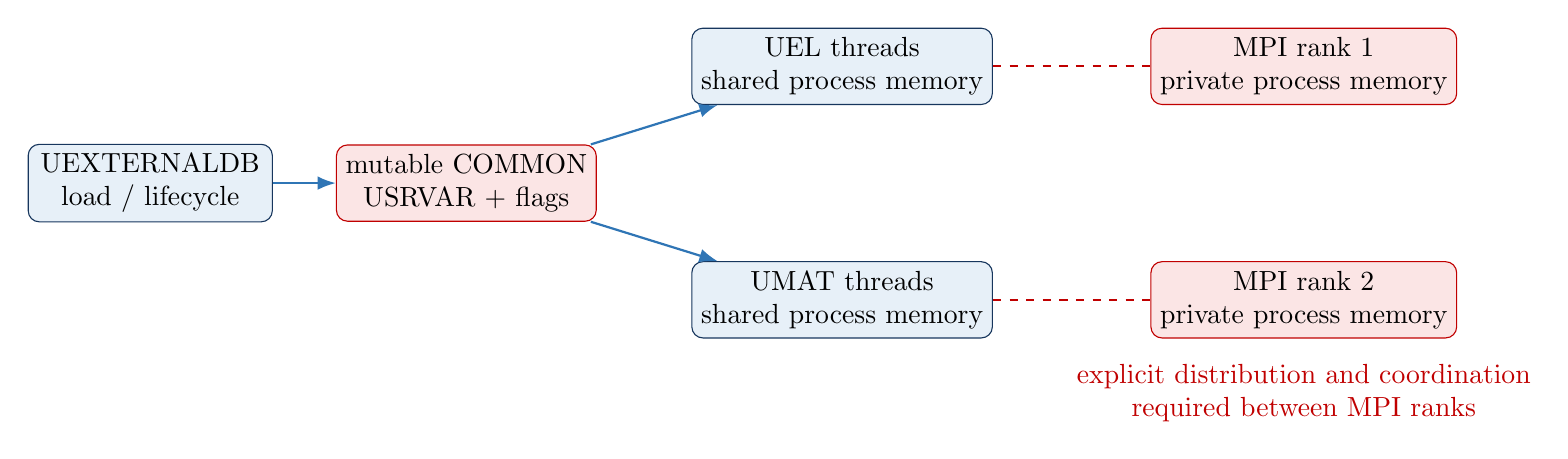
\begin{tikzpicture}[node distance=8mm,box/.style={draw=navy,rounded corners,fill=pb,minimum width=31mm,minimum height=9mm,align=center},risk/.style={draw=red,fill=pr,rounded corners,minimum width=31mm,minimum height=9mm,align=center},arr/.style={-{Latex},thick,blue}]
\node[box](ext){UEXTERNALDB\\load / lifecycle};\node[risk,right=of ext](com){mutable COMMON\\USRVAR + flags};
\node[box,above right=5mm and 12mm of com](uel){UEL threads\\shared process memory};\node[box,below right=5mm and 12mm of com](umat){UMAT threads\\shared process memory};
\node[risk,right=20mm of uel](mpi){MPI rank 1\\private process memory};\node[risk,right=20mm of umat](mpi2){MPI rank 2\\private process memory};
\draw[arr](ext)--(com);\draw[arr](com)--(uel);\draw[arr](com)--(umat);\draw[dashed,red,thick](uel)--(mpi);\draw[dashed,red,thick](umat)--(mpi2);
\node[below=2mm of mpi2,text=red,align=center]{explicit distribution and coordination\\required between MPI ranks};
\end{tikzpicture}}
\end{center}
\footnotesize\textbf{Figure 6.} Current risk model: thread memory sharing and MPI process separation create different qualification obligations. Source: Stage-P static shared-state audit and Abaqus 2023 utility-interface evidence.\par
\normalsize
The Stage-P static audit found 38 COMMON, 7 SAVE, 21 DATA, and 87 WRITE occurrences across the audited variants. USRVAR is read/written from UEL and UMAT, and UEXTERNALDB variants perform shared-state loading and file I/O. Static inspection identifies risk; it cannot prove callback order, same-thread ownership, or cross-rank consistency.

\clearpage\headx{8. Parallelization evidence and current status}
\small
\begin{tabularx}{\linewidth}{@{}p{29mm}p{38mm}Xp{29mm}@{}}\toprule
Execution mode&Abaqus capability / memory model&Current implementation evidence&Status\\\midrule
Serial&ordinary user-subroutine baseline&P3-S failed with signal 11; minimized P3-SM0 and later serial identifier lanes completed; finalized P3-SB evidence retained&\colorbox{green}{\textcolor{white}{\bfseries\tiny SERIAL BASELINE}}\\
1 MPI rank, 4 threads&threads share process state&D2C tiny case matched accepted continuation; positive case-specific repeatability only. P3-T4 failed compilation before callbacks/solver.&\status{amber}{CASE EVIDENCE}\\
Multiple MPI ranks&separate rank address spaces&no proof that COMMON/global state is distributed consistently&\status{gray}{UNQUALIFIED}\\
Hybrid MPI + threads&both risk classes apply&no valid scientific hybrid evidence&\status{gray}{UNTESTED}\\\bottomrule
\end{tabularx}
\normalsize
P3-S was diagnostic rather than a valid parallel qualification. P3-SM0 isolated a minimal callback; P3-SM1 variants established usable identifier-call routes in serial. P3-T4 job 1378242 exited during Intel compilation because the Abaqus utility header was placed outside a valid Fortran program unit. No link, input processing, callback diagnostics, ODB, or scientific comparison occurred. Consequently it supplies no threaded safety result.

\boxx{pg}{\textbf{Positive evidence.} D2C shows equality for one tiny one-rank/four-thread case. This is useful repeatability evidence.}
\boxx{pr}{\textbf{Claim boundary.} Abaqus parallel modes being available does not mean this mutable COMMON/SAVE implementation is safe in them. General thread safety, MPI state consistency, and hybrid safety remain separate, unqualified claims.}

\clearpage\headx{9. Proposed parallelization subproblem}
The next investigation should proceed as a gated engineering subproblem, with no promise of production parallel speedup before numerical equality and determinism are demonstrated.
\small
\begin{tabularx}{\linewidth}{@{}p{13mm}p{47mm}X@{}}\toprule
Stage&Action&Measurable output / pass condition\\\midrule
P-A&Static shared-state and file-I/O inventory&owner, writer, lifecycle, rank/thread scope for every mutable value\\
P-B&Frozen serial deterministic baseline&repeat RF--U, SDV14/15/16, phase, history ordering, energy and hashes\\
P-C&One-rank multithread characterization&numerical equality, repeated-run determinism, callback/access trace\\
P-D&Thread-safe refactor&remove or synchronize unsafe mutable writes; repeat P-B/P-C gates\\
P-E&Multi-rank distribution design&partition/replicate state explicitly; prove rank-complete ordering and equality\\
P-F&Hybrid test&equality plus deterministic runtime, speedup and memory scaling\\\bottomrule
\end{tabularx}
\normalsize
For every stage, compare the complete RF--U curve, SDV14/15/16 fields, history ordering, phase irreversibility, energies, deterministic repeat hashes/tolerances, wall/CPU time, and peak memory. Compile/link qualification precedes solver execution; case-specific equality does not silently generalize to another mesh, thread count, or MPI decomposition.

\boxx{pb}{\textbf{Direct answer.} The limitation is best understood as an implementation thread-safety and inter-rank-state problem, not as ``UEXTERNALDB forbids parallelism.'' The present code nevertheless remains serial-qualified only, with one small case-specific threaded repeat; refactoring and staged tests are required before parallel production use.}

\clearpage\headx{10. Claim matrix: 24 July versus 11 August}
\footnotesize
\begin{tabularx}{\linewidth}{@{}p{29mm}p{24mm}p{27mm}Xp{29mm}@{}}\toprule
Claim&24 July&11 August&Evidence&Remaining limitation\\\midrule
MISESERI pre-refinement&validated in scope&SUPPORTED&offline/native candidate generation&indicator is not fracture solution\\
Uniform verification&partial Mode-I roles&PASS pre-peak&H2 scheduler ambiguity resolved; jobs 1386372, 1386447, 1388330&H1/H2 diverge before endpoint; peak convergence unresolved\\
Adaptive global response&pre-peak refined-v3&SUPPORTED&1386469/70; $\sim0.16\%$ MM/PK5 RF&not crack convergence\\
Adaptive crack path&not equivalent&FAIL gate&H1/H2 matched Hausdorff 0.005443 mm&gate 0.003750 mm\\
Nonmatching transfer&bounded offline/ingestion&artifact exists&MM-to-artifact mapping&runtime chain fails\\
Mechanical restart&unproven&FAIL audit&1386471 reproduced virgin PK5&requires explicit ingestion\\
Runtime ingestion&bounded older test only&FAIL current path&UEL ignores SVARS/artifact&reader/init redesign\\
Evolving remesh&withheld&HOLD&Restart2 prepared but checkpoint invalid&dependent on ingestion proof\\
COMMON thread safety&not general&UNRESOLVED&D2C positive; static risks; P3-T4 compile fail&general equality absent\\
MPI / hybrid safety&not established&UNRESOLVED&no valid multi-rank/hybrid science&distribution design absent\\
Online remeshing&withheld&NOT YET CLAIMED&offline CAE remesh/candidate work only&no closed online loop\\\bottomrule
\end{tabularx}
\normalsize
\boxx{pg}{\textbf{Resolved or materially advanced.} Corrected FRACFIX/NPHYS formulation; H2 scheduler censoring resolved with exact old/new reproduction and an identified interior peak; scoped pre-peak uniform consistency; adaptive endpoint completion; and a precise parallel risk model.}
\boxx{pr}{\textbf{Still unresolved.} Complete uniform post-peak reference, crack-path convergence, actual transferred-state restart, second evolving remesh, online loop, and general parallel safety.}

\clearpage\headx{11. Limitations and the next 2--4 weeks}
\textbf{Current limitations.} H1 and H2 both terminate by numerical divergence before the prescribed endpoint; H2 scheduler censoring is resolved, but global peak and full post-peak convergence remain unresolved because H1 is incomplete. The frozen crack-path gate fails, no complete uniform reference exists, direct validated fracture-energy history is unavailable, and H2 contains eight small SDV15 decreases. Runtime state ingestion fails and Restart2 is on hold. Native/offline mesh creation is not an online loop. General thread, MPI, and hybrid safety remain unresolved.

\begin{minipage}[t]{.48\linewidth}
\boxx{pb}{\textbf{Scientifically required}
\begin{enumerate}
\item Implement and prove artifact-to-target runtime initialization for nodal phase and integration-point history.
\item Re-run only after fresh qualification/authorization, then verify source $\rightarrow$ artifact $\rightarrow$ first solver state.
\item If that passes, perform one controlled second evolving-remesh transfer and matched-state audit.
\item Consolidate RF--U, field, energy, crack geometry, cost, and censoring in the thesis.
\item Complete P-A/P-B and design the thread-safe state boundary before further parallel tests.
\end{enumerate}}
\end{minipage}\hfill
\begin{minipage}[t]{.48\linewidth}
\boxx{pa}{\textbf{Optional sensitivity work}
\begin{enumerate}
\item Additional corridor refinement only if the matched-state crack metric motivates it.
\item Alternative transfer projection only after runtime ingestion is proven.
\item MPI/hybrid performance study only after equality and determinism gates pass.
\item No further H2 rerun: the endpoint-resolution experiment has achieved its purpose.
\end{enumerate}}
\end{minipage}
\boxx{pr}{\textbf{Stop condition.} Do not execute Restart2 or claim evolving/online remeshing until the executable initialization path consumes the state and the first solver state is independently verified.}

\clearpage\headx{12. Reproducibility appendix}
\small
\begin{tabularx}{\linewidth}{@{}p{32mm}X@{}}\toprule
Item&Frozen identity or location\\\midrule
Report evidence revision&\texttt{d2c9c6a6d5f8dce94924ecb9cf6ab77fec96d7be}\\
Current production UEL SHA-256&\texttt{0bc4378179a35acd9954d20d3e07517f8e1c356ae07a23c40e7715cd7b56dce8}\\
Uniform jobs&H0 \texttt{1386372}; H1 \texttt{1386447}; historical H2 \texttt{1386448}; endpoint-resolution H2 \texttt{1388330}\\
Adaptive jobs&MM \texttt{1386469} (M2ADAPT\_MM\_FRACFIX\_PROD); PK5 \texttt{1386470} (M2ADAPT\_PK5\_FRACFIX\_PROD)\\
Restart audit&\texttt{1386471} (M2STATE\_FRACFIX\_RESTART1); primary audit: {\ttfamily project\_coordination/sessions/\newline 2026-08-11\_0525\_gemini-antigravity\_\newline F43STATE-M2-RUNTIME-INGESTION-AUDIT1.md}; revision \texttt{d2c9c6a6d5f8dce94924ecb9cf6ab77fec96d7be}\\
Uniform evidence&\texttt{models/generated/mode\_ii/reference\_convergence/}; Pair-2 censoring audit\\
Adaptive evidence&\texttt{models/generated/mode\_ii/production\_adaptive\_batch/}\\
Transfer evidence&\texttt{models/generated/mode\_ii/production\_state\_transfer\_batch/}\\
Parallel evidence&\texttt{runs/hpc/stage\_p/}; \texttt{results/validation/stage\_p\_static\_audit/}\\
Software&Abaqus 2023; Intel 2024.2.0 and GCC 11.4.0 environment; Abaqus Python runtime; serial jobs reported here use one CPU\\\bottomrule
\end{tabularx}
\normalsize
\textbf{Evidence notes.} Numerical values come from primary scheduler/solver records, extracted curves, frozen comparison contracts, endpoint closeout, and the executable-path audit. H2 has a defensible interior peak; cross-mesh global peak convergence remains unresolved because H1 is incomplete. H0/H2 available-domain RF $L_2=1.891\%$ and work difference $=1.304\%$ through 0.0097625 mm are contextual, not full-path convergence. The report does not expose credentials or reproduce bulky solver artifacts.

\vfill
\boxx{pb}{\textbf{Current claim boundary in one sentence.} The work now supports scoped Mode-II pre-peak uniform consistency and endpoint-complete, globally agreeing low-cost adaptive solutions, but it does not yet support converged crack geometry, actual nonmatching runtime state ingestion, a second evolving remesh, online adaptivity, or generally safe parallel execution.}
\end{document}
